% ****** Start of file apssamp.tex ******
%
%   This file is part of the APS files in the REVTeX 4.1 distribution.
%   Version 4.1r of REVTeX, August 2010
%
%   Copyright (c) 2009, 2010 The American Physical Society.
%
%   See the REVTeX 4 README file for restrictions and more information.
%
% TeX'ing this file requires that you have AMS-LaTeX 2.0 installed
% as well as the rest of the prerequisites for REVTeX 4.1
%
% See the REVTeX 4 README file
% It also requires running BibTeX. The commands are as follows:
%
%  1)  latex apssamp.tex
%  2)  bibtex apssamp
%  3)  latex apssamp.tex
%  4)  latex apssamp.tex
%
\documentclass[%
 reprint,	
%superscriptaddress,
%groupedaddress,
%unsortedaddress,
%runinaddress,
%frontmatterverbose, 
%preprint,
showpacs,
% preprintnumbers,
%nofootinbib,
%nobibnotes,
%bibnotes,
 amsmath,amssymb,
 aps,
 superscriptaddress,
%prl,
%prc,
%prb,
%rmp,
%prstab,
%prstper,
%floatfix,
]{revtex4-1}

\usepackage{graphicx}% Include figure files
\usepackage{dcolumn}% Align table columns on decimal point
\usepackage{bm}% bold math
\usepackage{url}
\usepackage{lipsum}
\usepackage{color}
\usepackage{hyperref}% add hypertext capabilities
\usepackage[mathlines]{lineno}% Enable numbering of text and display math
\usepackage{upgreek}
\usepackage{biolinum}
\linenumbers\relax % Commence numbering lines

%\usepackage[showframe,%Uncomment any one of the following lines to test 
%%scale=0.7, marginratio={1:1, 2:3}, ignoreall,% default settings
%%text={7in,10in},centering,
%%margin=1.5in,
%%total={6.5in,8.75in}, top=1.2in, left=0.9in, includefoot,
%%height=10in,a5paper,hmargin={3cm,0.8in},
%]{geometry}

% \setcounter{secnumdepth}{5}
\begin{document}

\preprint{APS/123-QED}

\title{Probing Strangeness Canonical Ensemble with $K^{-}$, $\phi(1020)$ and $\Xi^{-}$ Production in Au+Au Collisions at ${\sqrt{s_{\rm NN}} = \rm{3\,GeV}}$: Supplemental Material}% Force line breaks with \\
%\thanks{A footnote to the article title}%

% \author{Ann Author}
% \altaffiliation[Also at ]{Physics Department, XYZ University.}%Lines break automatically or can be forced with \\
% \author{Second Author}%
% \email{Second.Author@institution.edu}
% \affiliation{% Authors' institution and/or address\\ This line break forced with \textbackslash\textbackslash
% }%
\input{star-author-list-2021-06-22.aps.tex}

\date{\today}% It is always \today, today,
             %  but any date may be explicitly specified


%\begin{description}
%\item[Usage]
%Secondary publications and information retrieval purposes.
%\item[PACS numbers]
%May be entered using the \verb+\pacs{#1}+ command.
%\item[Structure]
%You may use the \texttt{description} environment to structure your abstract; use the optional argument of the \verb+\item+ command to give the category of each item. 
%\end{description}

%\pacs{25.75.-q, 25.75.Cj}% PACS, the Physics and Astronomy
                             % Classification Scheme.
%\keywords{Suggested keywords}%Use showkeys class option if keyword
                              %display desired
\maketitle

% Chapter one
% \section{Introduction}
% \label{introduction}

% \bibliography{phi3GeV.bib}

% \newpage
% \vspace{5.0cm}

\section{supplemental material}

\subsection{Full Corrected $m_T$ Spectra}

Figure~\ref{fig:phimTSpectra21} shows the corrected $K^-$, $\phi$ meson and $\Xi^-$ invariant yields as a function of $m_T-m_0$ for various rapidity ranges in 0--10\% (left) and 10--40\% (right) centrality Au+Au collisions at ${\sqrt{s_{\rm NN}} = \rm{3\,GeV}}$. The $K^-$, $\phi$-meson and $\Xi^-$ spectra in some rapidity intervals are scaled with arbitrary factors indicated in the figure for clarity. Dashed and solid lines depict fits to the spectra with the $m_T$-exponential function in order to extrapolate the unmeasured $p_T$ ranges. Figure~\ref{fig:phimTSpectra23} shows the similar plot for $K^-$ and $\phi$ meson in 40--60\% centrality Au+Au collisions.

\begin{figure*}
\centering
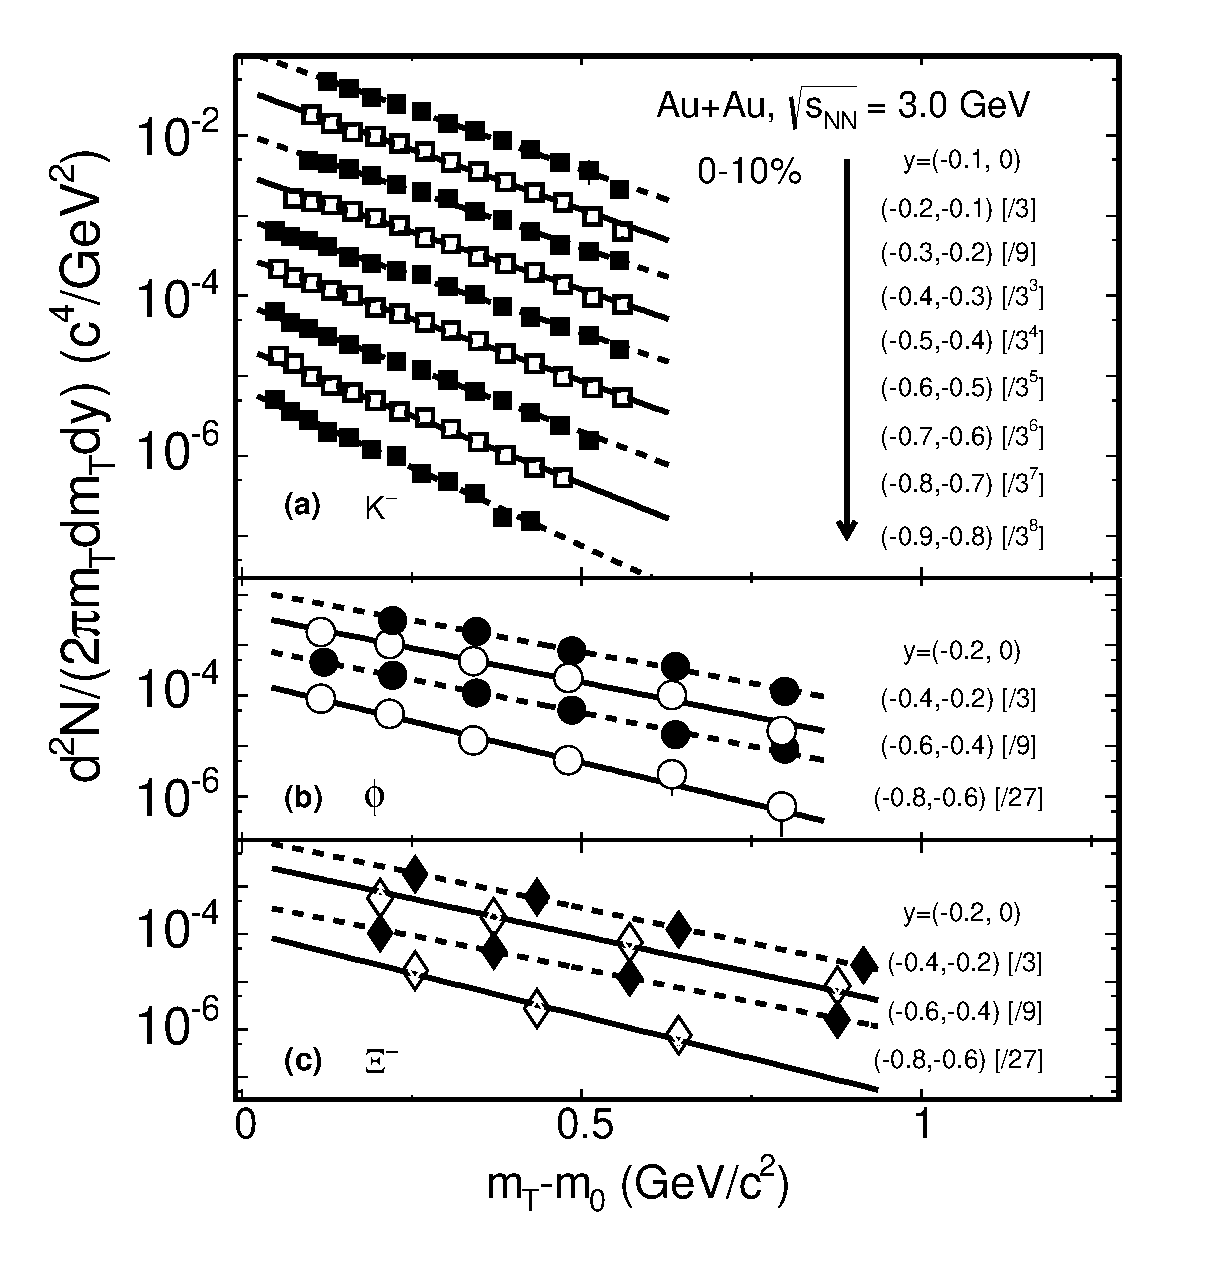
\includegraphics[width=0.43\textwidth]{fig21.eps}
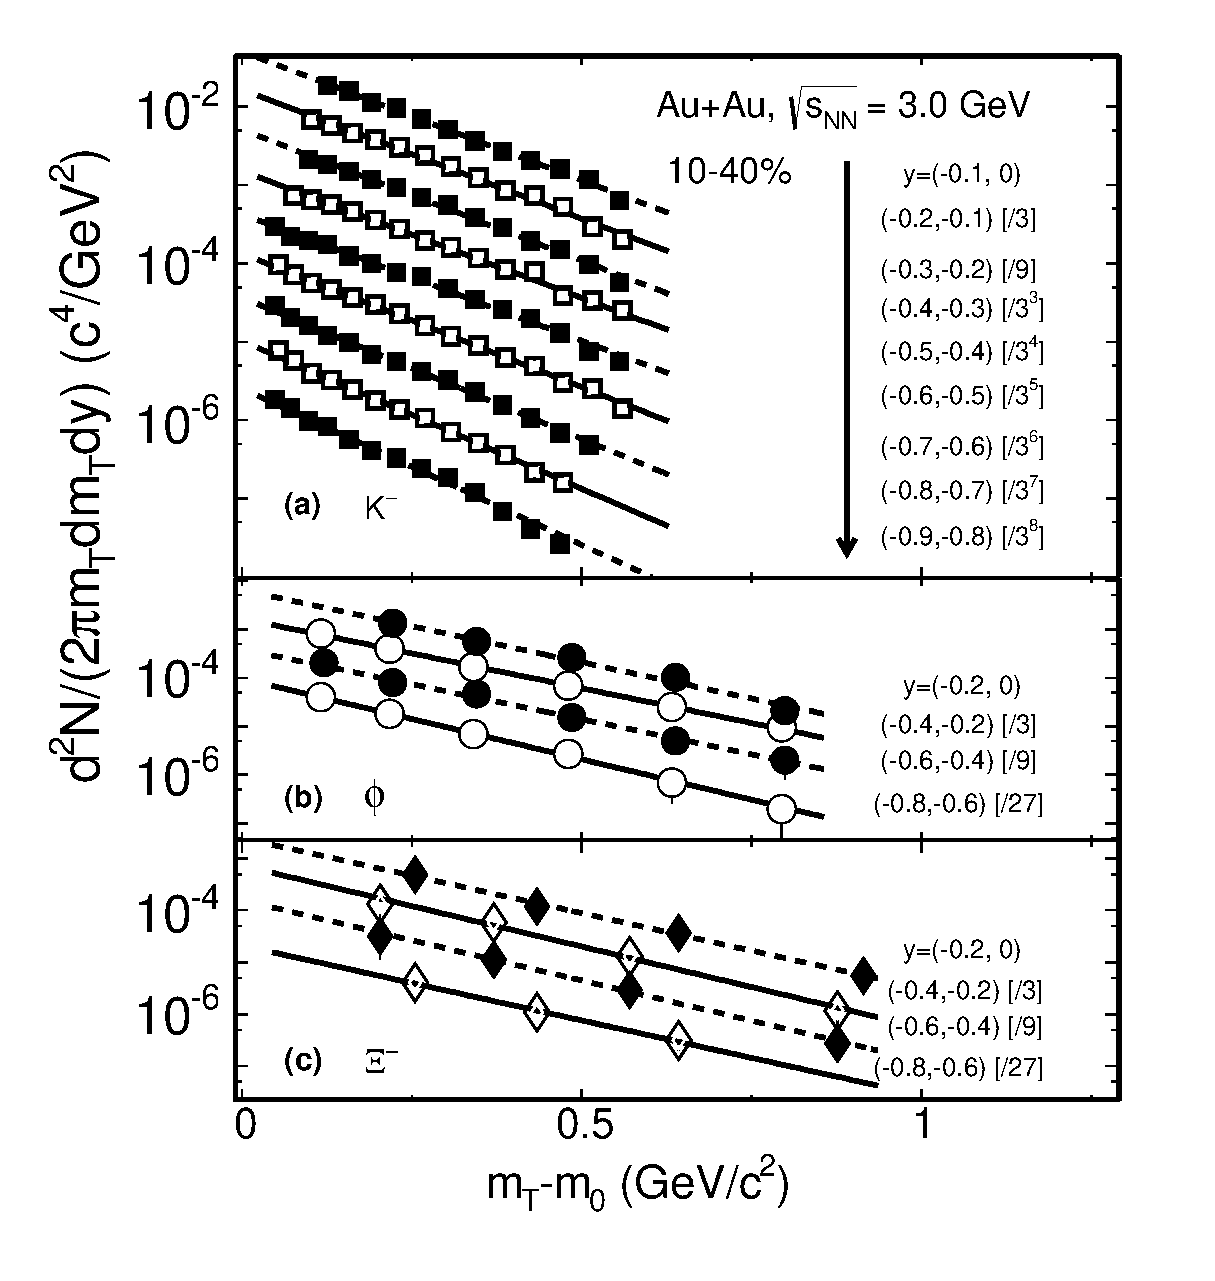
\includegraphics[width=0.43\textwidth]{fig22.eps}
\caption{$K^-$ (a), $\phi$ meson (b) and $\Xi^-$ (c) invariant yields as a function of $m_T-m_0$ for various rapidity regions in 0--10\% (left) and  10--40\% (right) centrality Au+Au collisions at ${\sqrt{s_{\rm NN}} = \rm{3\,GeV}}$. Statistical and systematic uncertainties are added quadratically here for plotting. Solid and dashed black lines depict $m_T$ exponential function fits to the measured data points with scaling factors in each rapidity windows.}
\label{fig:phimTSpectra21}
\end{figure*}

\begin{figure}
\centering
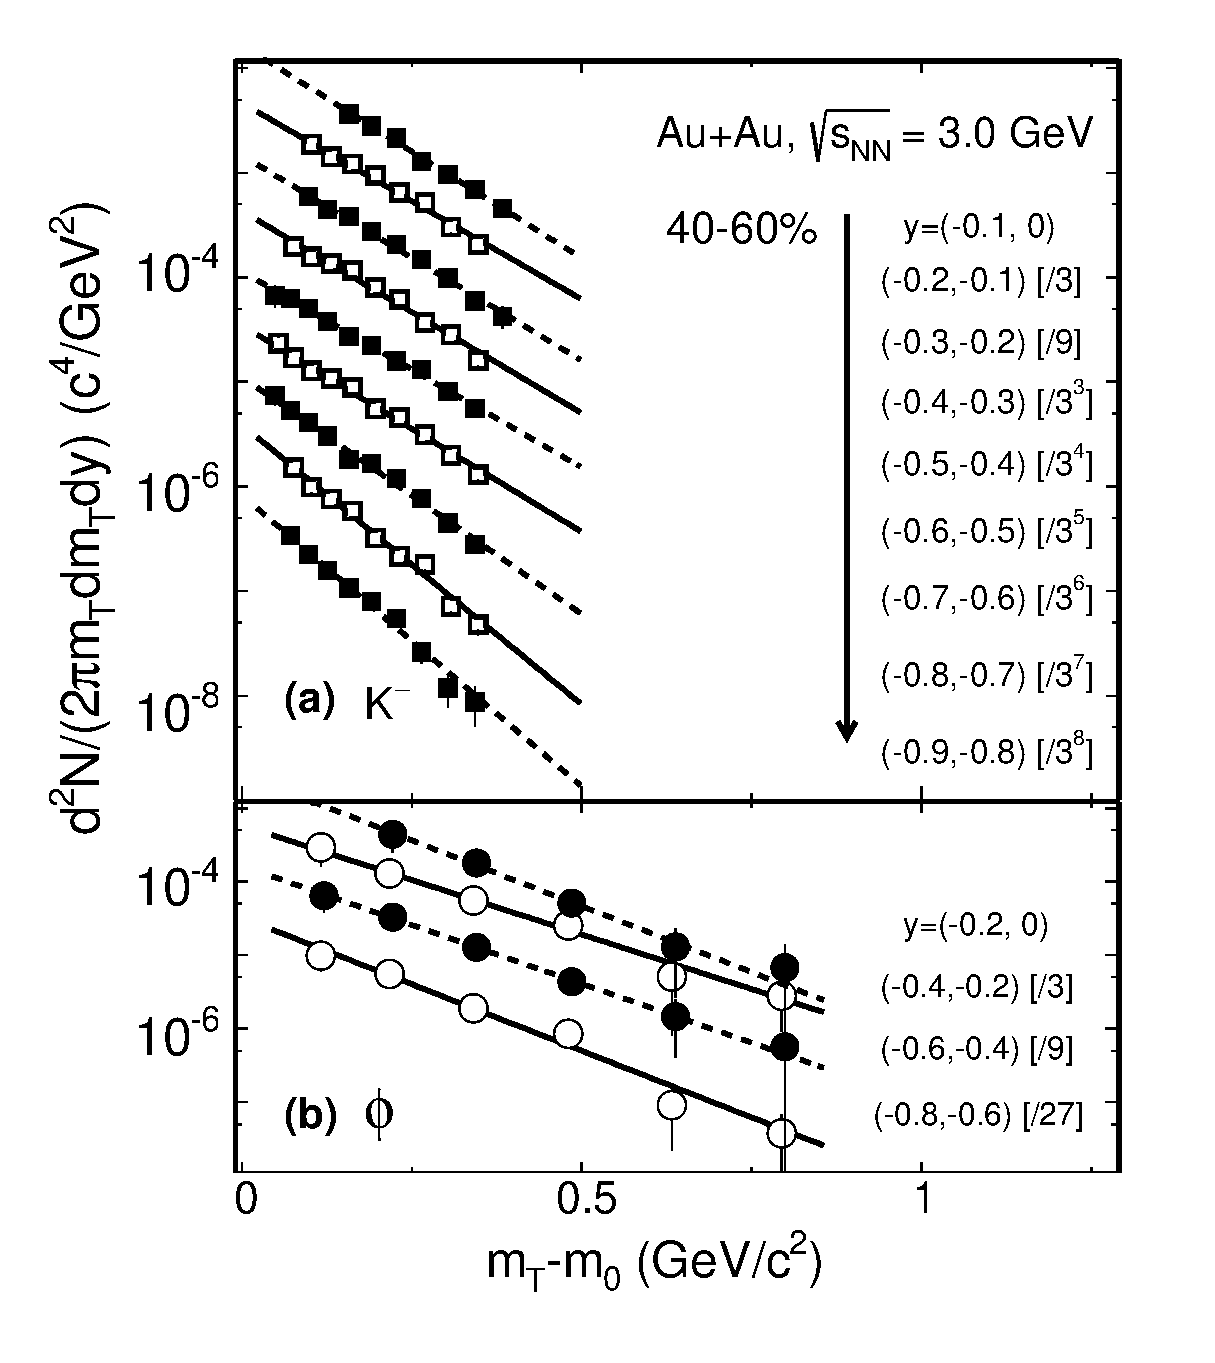
\includegraphics[width=0.43\textwidth]{fig23.eps}
\caption{$K^-$ (a) and $\phi$ meson (b) invariant yields as a function of $m_T-m_0$ for various rapidity regions in 40--60\% centrality Au+Au collisions at ${\sqrt{s_{\rm NN}} = \rm{3\,GeV}}$.}
\label{fig:phimTSpectra23}
\end{figure}


\end{document}
%
% ****** End of file apssamp.tex ******
